\section{Output Distribution of raw audio WaveNet models}\label{appx:wavenet-output-distribution}
\begin{figure}[ht]
    \centering
    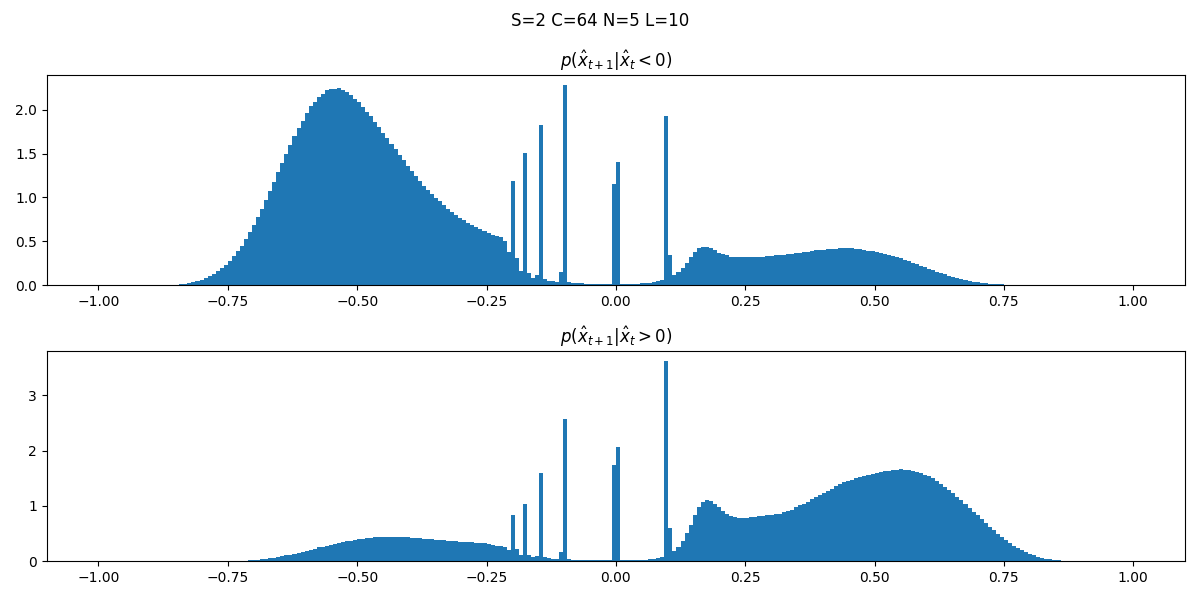
\includegraphics[width=0.45\textwidth]{gfx/S2_N5_L10_C64_output_distribution.png}
    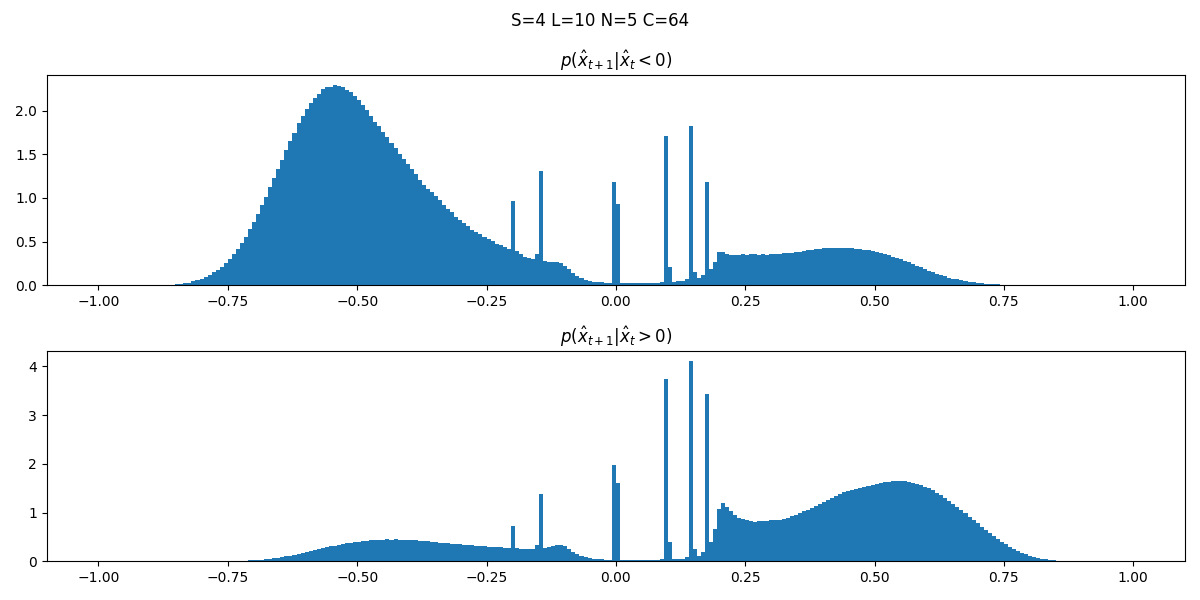
\includegraphics[width=0.45\textwidth]{gfx/S4_N5_L10_C64_output_distribution.png}
    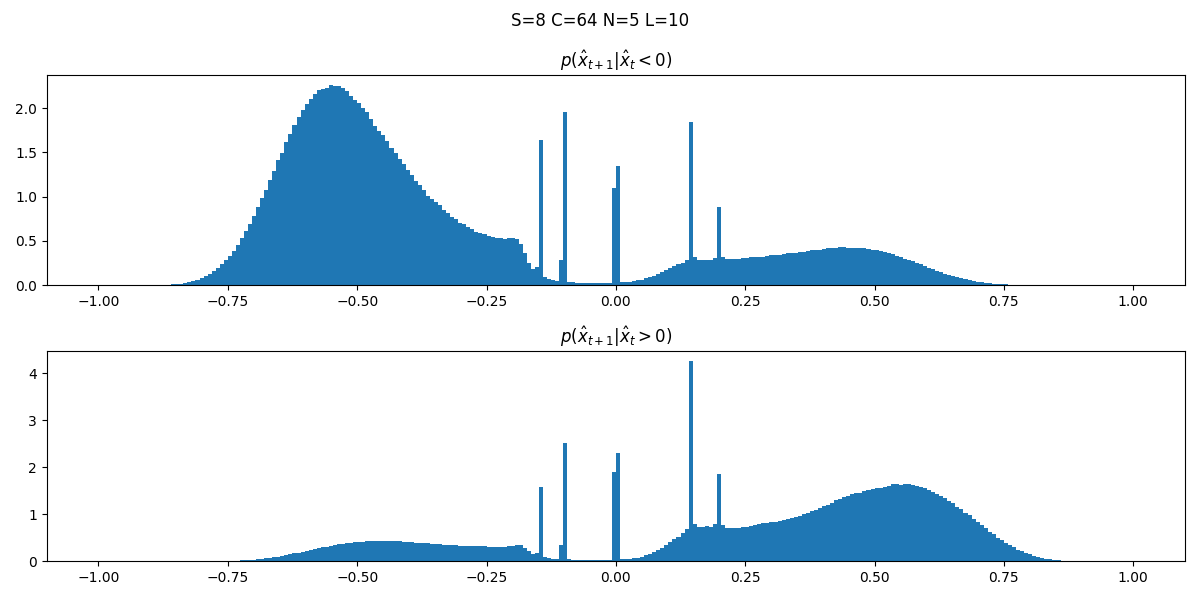
\includegraphics[width=0.45\textwidth]{gfx/S8_N5_L10_C64_output_distribution.png}
    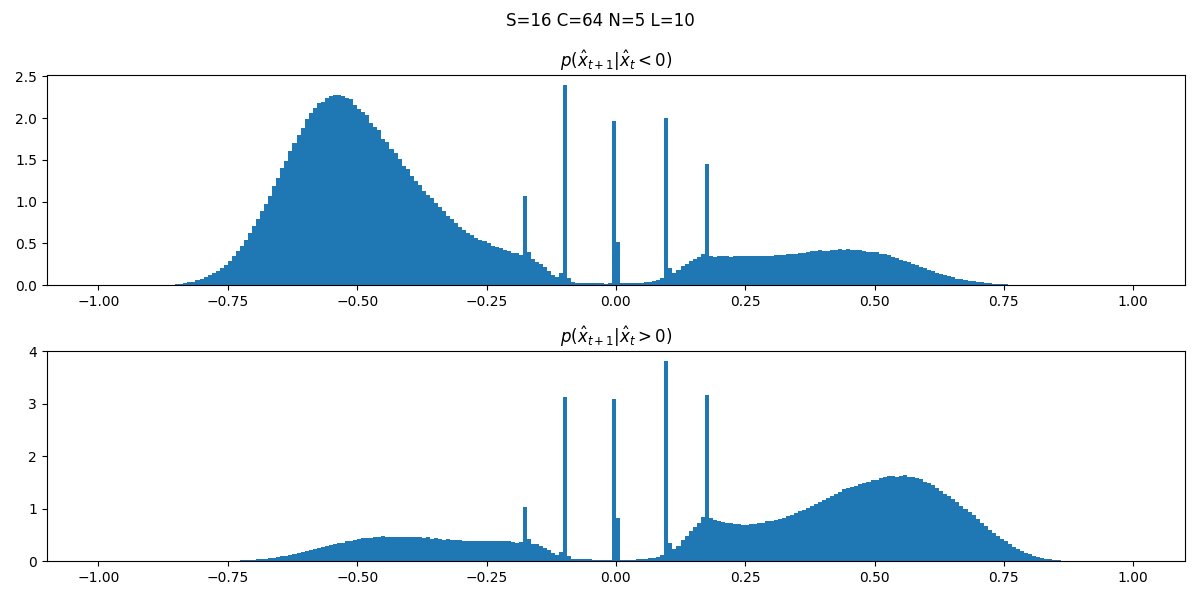
\includegraphics[width=0.45\textwidth]{gfx/S16_N5_L10_C64_output_distribution.png}
    \caption{
    Sampled Output Distributions for WaveNet models trained on the Librispeech \texttt{clean-100h} subset.
    Distributions are in 16 bit $\mu$-law space and binned into 256 bins from -1 to 1.
    }
    \label{fig:wavenet-output-distributions}
\end{figure}


\begin{figure}[ht]
    \centering
    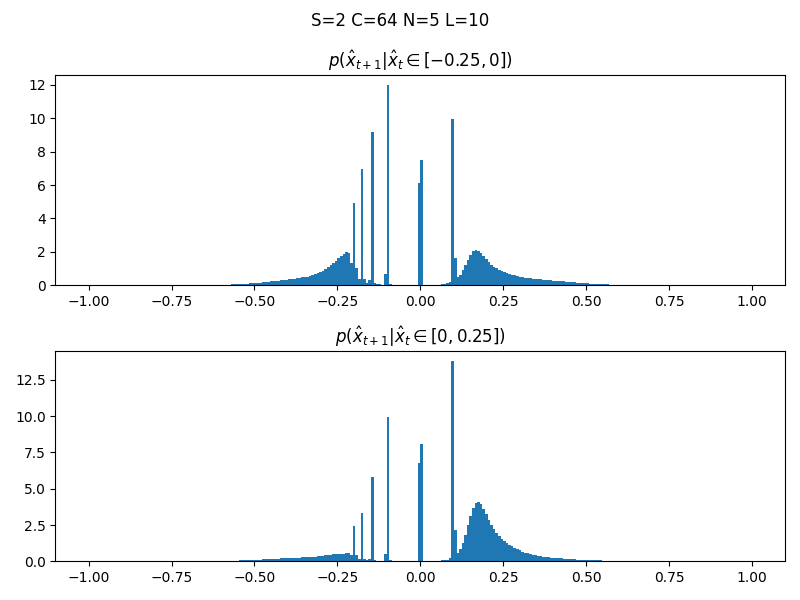
\includegraphics[width=0.45\textwidth]{gfx/S2_N5_L10_C64_output_distribution_cut.png}
    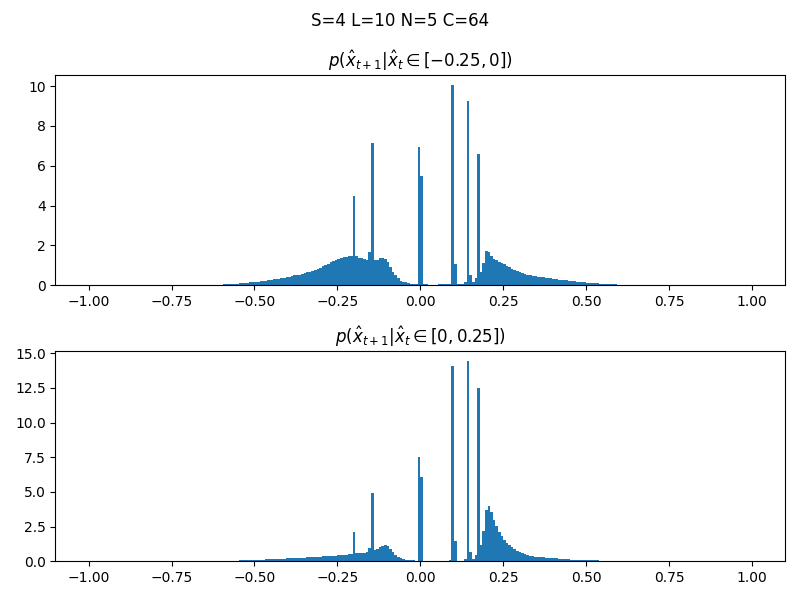
\includegraphics[width=0.45\textwidth]{gfx/S4_N5_L10_C64_output_distribution_cut.png}
    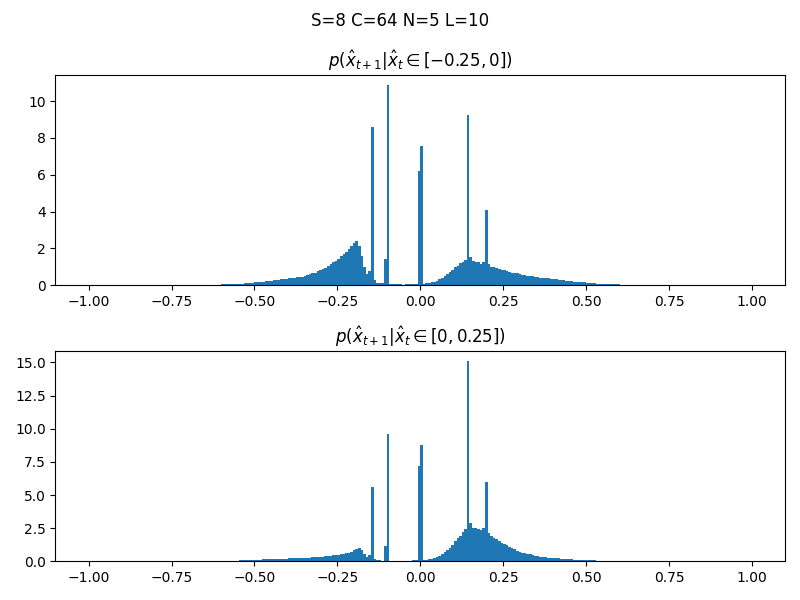
\includegraphics[width=0.45\textwidth]{gfx/S8_N5_L10_C64_output_distribution_cut.png}
    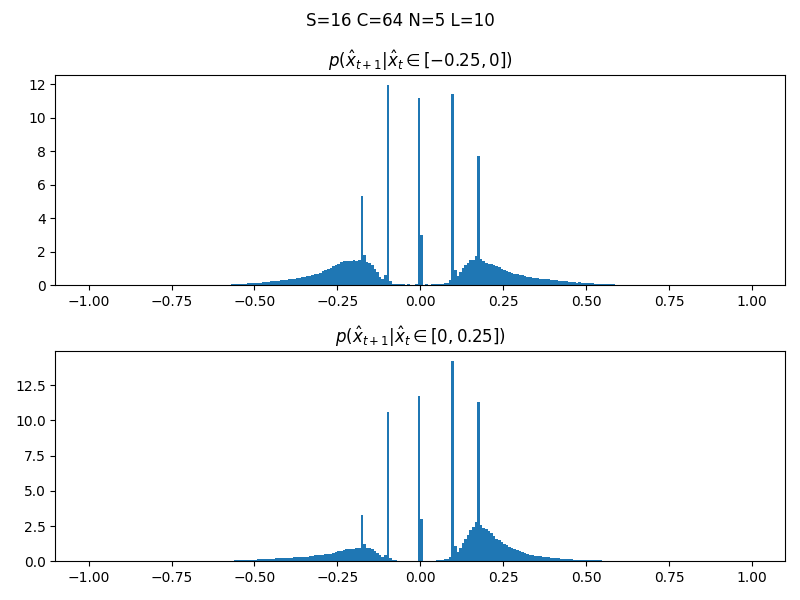
\includegraphics[width=0.45\textwidth]{gfx/S16_N5_L10_C64_output_distribution_cut.png}
    \caption{
    Sampled Output Distributions for WaveNet models trained on the Librispeech \texttt{clean-100h} subset.
    Distributions are in 16 bit $\mu$-law space and binned into 256 bins from -1 to 1.
    }
    \label{fig:wavenet-output-distributions-cut}
\end{figure}

In \cref{fig:wavenet-output-distributions} we plot following output distributions for each model:
\[
p(\hat{x}_{t+1} | \hat{x}_{t} < 0 )
\\
p(\hat{x}_{t+1} | \hat{x}_{t} > 0 )
\]
Likewise, in \cref{fig:wavenet-output-distributions-cut} we plot a more constrained output distribution:
\[
p(\hat{x}_{t+1} | \hat{x}_{t} \in [-0.25, 0] )
\\
p(\hat{x}_{t+1} | \hat{x}_{t}  \in [0, 0.25] )
\]


From these we see:
\begin{itemize}
    \item A clear tendency to predict samples with the same sign as $x_t$, as expected.
    \item A multimodality, assigning non-zero probability to sample the opposite sign. This gives clear support that WaveNet's output distribution learns characteristic features of audio sequences, even when predicting multiple timesteps simultaneously.
    \item Some overespresented peaks close to 0. We attribute these to the stretching of values close to 0 from a $\mu$-law transform. A similar phenomenon is seen when transforming the TIMIT dataset in \cref{fig:mu-law-enc}, far right.
\end{itemize}